\documentclass[11  pt]{article} 
\usepackage[lmargin=1in,rmargin=1.75in,bmargin=1in,tmargin=1in]{geometry}  


% For hyperlinking everything
\usepackage{hyperref}
\hypersetup{
	colorlinks=true, %set true if you want colored links
	linktoc=all,     %set to all if you want both sections and subsections linked
	linkcolor=blue,  %choose some color if you want links to stand out
}


\usepackage[latin1]{inputenc}
\usepackage{amsmath}
\usepackage{mathrsfs}  
\usepackage{amsfonts}
\usepackage{amssymb}
\usepackage{graphicx}
\usepackage{subfig}
\usepackage{caption}
\usepackage{algorithm}
%\usepackage{algcompatible}
%\usepackage{algorithmicx}
\usepackage{algpseudocode}

\usepackage{titlesec}
\titleformat{\section}{\fontfamily{lmss}\fontsize{14}{15}\bfseries}{\thesection}{1em}{}
\titleformat{\subsection}{\fontfamily{lmss}\fontsize{12}{15}\bfseries}{\thesubsection}{1em}{}




\usepackage{amsthm}

\newtheoremstyle{noit}
{10pt}% <Space above>
{10pt}% <Space below>
{}% <Body font>
{}% <Indent amount>
{\bfseries}% <Theorem head font>
{.}% <Punctuation after theorem head>
{.5em}% <Space after theorem headi>
{}% <Theorem head spec (can be left empty, meaning `normal')>

\newtheoremstyle{example}
{10pt}% <Space above>
{10pt}% <Space below>
{}% <Body font>
{20pt}% <Indent amount>
{\bfseries}% <Theorem head font>
{.}% <Punctuation after theorem head>
{.5em}% <Space after theorem headi>
{}% <Theorem head spec (can be left empty, meaning `normal')>


\newtheoremstyle{indented}{20pt}{20pt}{\addtolength{\leftskip}{2.5em}}{}{\bfseries}{.}{.5em}{}


\newtheorem{theorem}{Theorem}
\numberwithin{theorem}{section}
\newtheorem{lemma}[theorem]{Lemma}
\newtheorem{corollary}[theorem]{Corollary}
\newtheorem{observation}{Observation}
%\numberwithin{observation}{section}
%\numberwithin{definition}{section}
\newtheorem{conjecture}{Conjecture}
\newtheorem{Qu}{Question}
\newcommand{\QU}{\begin{Qu}\normalfont}

\theoremstyle{noit}
\newtheorem{fact}{Fact}
\newtheorem{definition}{Definition}

\theoremstyle{indented}
\newtheorem{example}{Example}

\theoremstyle{indented}
\newtheorem{problem}{Problem}


%\newenvironment{proof}{\noindent{\bf Proof:} \hspace*{1em}}{
%    \hspace*{\fill} $\Box$ }
%\newenvironment{proof_of}[1]{\noindent {\bf Proof of #1:}
%    \hspace*{1em} }{\hspace*{\fill} $\Box$ }
%\newenvironment{proof_claim}{\begin{quotation} \noindent}{
%    \hspace*{\fill} $\diamond$ \end{quotation}}
\newcommand{\vs}[1]{\vspace{#1}}

\newcommand{\lecture}[2]{
 \noindent
\begin{center}
	\framebox{
		\vbox{
			\hbox to 5.78in { {\bf CSCE 411: Design and Analysis of Algorithms} \hfill  }
			\vspace{2mm}
			\hbox to 5.78in { {\Large \hfill Lecture #1\hfill} }
			\vspace{2mm}
			\hbox to 5.78in { {\it Date: #2 \hfill Lecturer: Nate Veldt} }
		}
	}
\end{center}
\vspace*{4mm}
}


\newcommand{\hw}[2]{
	\noindent
	\begin{center}
		\framebox{
			\vbox{
				\hbox to 5.78in { {\bf CSCE 411: Design and Analysis of Algorithms} \hfill  }
				\vspace{2mm}
				\hbox to 5.78in { {\Large \hfill Homework #1\hfill} }
				\vspace{2mm}
				\hbox to 5.78in { {\it Due date: #2 \hfil} }
			}
		}
	\end{center}
	\vspace*{4mm}
}



\newcommand{\under}[1]{\underline{\hspace{#1}}}
\setlength{\parindent}{0em}

%\usepackage[tagged]{accessibility}

% Graph terms
\newcommand{\vol}{\textbf{vol}}
\newcommand{\cut}{\textbf{cut}}


% Matrices
\newcommand{\mA}{\textbf{A}}
\newcommand{\mB}{\textbf{B}}

% vectors
\newcommand{\ve}{\textbf{e}}
\newcommand{\vx}{\textbf{x}}


% Other
\newcommand{\calN}{\mathcal{N}}

\usepackage{mathtools}
\DeclarePairedDelimiter\ceil{\lceil}{\rceil}
\DeclarePairedDelimiter\floor{\lfloor}{\rfloor}


\newcommand*{\aitem}{ \item[{
\includegraphics[width=0.8cm,height=0.5cm]{../../Lectures/figures/A}} ]  }
\newcommand*{\bitem}{ \item[{
\includegraphics[width=0.8cm,height=0.5cm]{../../Lectures/figures/B}} ]  }
\newcommand*{\citem}{ \item[{
\includegraphics[width=0.8cm,height=0.5cm]{../../Lectures/figures/C}} ]  }
\newcommand*{\ditem}{ \item[{
\includegraphics[width=0.8cm,height=0.5cm]{../../Lectures/figures/D}} ]  }
\newcommand*{\eitem}{ \item[{
\includegraphics[width=0.8cm,height=0.5cm]{../../Lectures/figures/E}} ]  }
\newcommand*{\fitem}{ \item[{
\includegraphics[width=0.8cm,height=0.5cm]{../../Lectures/figures/F}} ]  }


\newcommand{\hide}[1]{\underline{\phantom{#1 #1}}}

\usepackage{setspace}

\onehalfspacing

\begin{document}
	
	\lecture{: Approximation Algorithms and Optimization}{Week 14}
	\textbf{Course Logistics}
	\begin{itemize}
		\item CLRS Chapter 34
		\item Last homework due Friday
	\end{itemize}
	
	
		\section{Linear programming}
		
		A linear program is a mathematical optimization problem with 
	\begin{itemize}
		\item A linear objective function
		\item Linear constraints
	\end{itemize}

We will use $x_i$ to denote variables---unknowns that we need to find to make the objective function as large as possible, and such that the constraints hold. \\

\paragraph{Examples} 

\newpage

		
		\paragraph{Warm-up problem (from CLRS).} 
As a politician seeking approval ratings, you would like the
support of 50 urban voters, 100 suburban voters, 25 rural
voters. 
		
For each $\$1$ spent advertising one of the following policies,
the resulting effects are:
		
\begin{center}
\begin{tabular}{|c|c|c|c|}
\hline
\textbf{Policy} & \textbf{Urban} & \textbf{Suburban} & \textbf{Rural} \\
\hline
Zombie apocalypse & -2 & +5 & -3 \\
Shark with lasers & +8 & +2 & -5 \\
Flying cars roads & 0 & 0 & +10 \\
Dolphins voting & +10 & 0 & -2 \\
\hline
\end{tabular}
\end{center}		

Minimize the amount spent to achieve the desired voter support. 
How can we write this as an algorithmic or mathematic problem?		


\vs{1cm}
Create variables:
\begin{itemize}
\item
Let \hide{$x_1$} be the money spent on ads for preparing for a zombie apocalypse
\item
Let \hide{$x_2$} be the money spent on ads for sharks with lasers
\item
Let \hide{$x_3$} be the money spent on ads for roads for flying cars
\item
Let \hide{$x_4$} be the money spent on ads for allowing dolphins to vote
\end{itemize}
Then the objective of the problem is:

\vs{2cm}
The constraints of the problem are: 

\vs{4cm}
		
	
\newpage

\paragraph{Another example problem.} 
The students of \textbf{CSCE 411} are managing their semester project portfolios, which involve three types of projects:

\begin{itemize}
    \item \textbf{Project A:} Basic Algorithms.
    \item \textbf{Project B:} Graph Algorithms.
    \item \textbf{Project C:} Complexity. 
\end{itemize}

Each project type earns a different amount of grade contribution points and consumes a mix of three limited resources: \textit{Self-Study Time}, \textit{Computation Credits}, and \textit{Team Collaboration Hours}.

\begin{center}
\begin{tabular}{|c|c|c|c|c|}
\hline
\textbf{Project Type} & \textbf{Grade Points} & \textbf{Time (hours)} & \textbf{Credits (units)} & \textbf{Collab Hours} \\
\hline
A & 10 & 5 & 3 & 2 \\
B & 12 & 6 & 2 & 4 \\
C & 8 & 4 & 4 & 3 \\
\hline
\end{tabular}
\end{center}

The semester budget for a student is:
\begin{itemize}
    \item Maximum 60 hours of Self-Study Time.
    \item Maximum 30 Computation Credits.
    \item Maximum 36 Collaboration Hours.
\end{itemize}

Additionally, the professor requires that at least 2 projects from each type be completed for a balanced learning experience.
Given the budget and these constraints, devise a project plan to maximize the grade. 

\vs{1cm}
Write a linear program for this problem.

\vfill
\newpage

%\section*{Linear Program (Primal Form)}
%
%Let:
%\begin{itemize}
    %\item \( x_1 \) = number of Project A completed.
    %\item \( x_2 \) = number of Project B completed.
    %\item \( x_3 \) = number of Project C completed.
%\end{itemize}
%
%The linear program is:
%
%\[
%\begin{aligned}
%\text{Maximize:} \quad & 10x_1 + 12x_2 + 8x_3 \\
%\text{Subject to:} \quad & 5x_1 + 6x_2 + 4x_3 \leq 60 \quad (\text{Time limit}) \\
%& 3x_1 + 2x_2 + 4x_3 \leq 30 \quad (\text{Computation credits limit}) \\
%& 2x_1 + 4x_2 + 3x_3 \leq 36 \quad (\text{Collaboration hours limit}) \\
%& x_1 \geq 2, \quad x_2 \geq 2, \quad x_3 \geq 2 \quad (\text{Minimum project count}) \\
%& x_1, x_2, x_3 \geq 0 \quad (\text{Non-negativity})
%\end{aligned}
%\]

\section{Types of Linear Programs}
Linear programs have many variations:
\begin{itemize}
	\item The objective function can be a maximization or a minimization problem
	\item The constraints can be equality or inequalities
	\item Often times, the variables will be greater than or equal to zero
\end{itemize}

If a particular solution $\overline{x}$ satisfies all of the constraints, we call it a \hide{feasible solution}. 
Otherwise, we call it an \hide{infeasible solution}.
The set of solutions that are feasible is called the \hide{feasible region}.

Actually, we can perform different conversions to

\begin{itemize}
	\item Turn a maximization problem into a minimization problem \\
	
	\vs{2cm}
	
	\item Turn an equality constraint into inequality constraints \\
	
		\vs{2cm}
	
	
	\item Turn an inequality constraint into an equality constraint \\
	
		\vs{2cm}
	
	\item Turn an unconstrained variable into positive variables \\
\end{itemize}


\vfill



\newpage
\section{Solving a Linear Program}
\textbf{Important Fact:} A linear program can be solved in polynomial time, e.g., the ellipsoid algorithm. 
There are other practical implementations, e.g., the simplex algorithm, that can run in exponential-time in the worst case. 

\vs{1cm}
Consider the linear program:

\[
\begin{aligned}
\text{Minimize:} \quad & x_1 + x_2 \\
\text{Subject to:} \quad & 4x_1 - x_2 \leq 8 \\
& 2x_1 + x_2 \leq 10 \\
& 5x_1 - 2x_2 \leq -2 \\
& x_1, x_2 \geq 0 \quad (\text{Non-negativity})
\end{aligned}
\]

\vs{1cm}
Intuition: The optimal solution must occur at a \hide{vertex} of the feasible region. 
\vfill
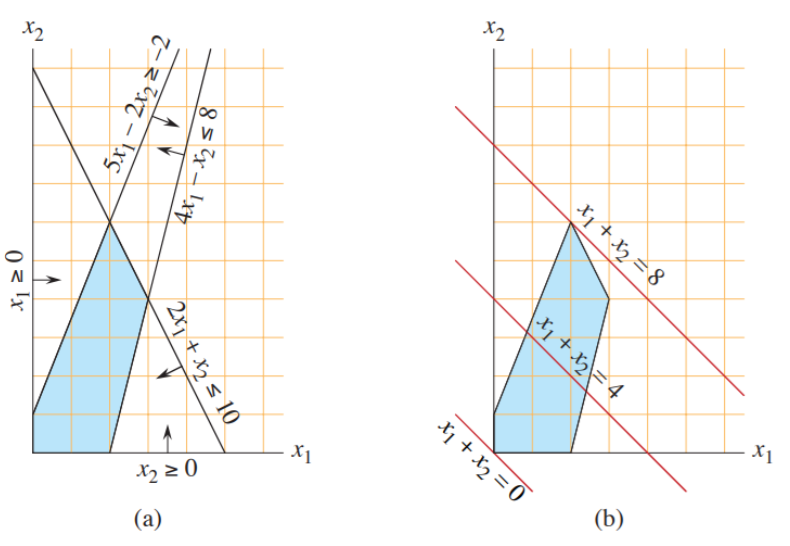
\includegraphics{lp-vertex.png}

\newpage

\section{Duality}

\QU
Consider the linear program:

\[
\begin{aligned}
\text{Maximize:} \quad & x_1 + 2x_2 + 3x_3 + 4x_4\\
\text{Subject to:} \quad & 10x_1 \leq 10 \\
& x_2 \leq 200 \\
& 5x_1 + 10x_2 + 15x_3 + 20x_4 \leq 15 \\
& x_1, x_2, x_3, x_4 \geq 0 \quad (\text{Non-negativity})
\end{aligned}
\]
What can we say about the optimal value? 
	\begin{itemize}
		\aitem $1$
		\bitem $3$ 
		\citem $10$
		\ditem $15$
		\eitem $200$
		\fitem The limit does not exist
	\end{itemize}
\end{Qu}

\newpage
Consider the linear program:

\[
\begin{aligned}
\text{Maximize:} \quad & 3x_1 + x_2 + 4x_3 \\
\text{Subject to:} \quad & x_1 + x_2 + 3x_3 \leq 30 \\
& 2x_1 + 2x_2 + 5x_3 \leq 24 \\
& 4x_1 + x_2 + x_3 \leq 36 \\
& x_1, x_2, x_3 \geq 0 \quad (\text{Non-negativity})
\end{aligned}
\]
What can we say about the optimal value? 

\vs{2cm}
What if we take the original constraints and add
the first two constraints?

\vs{2cm}
The primal solution must be at most \hide{54}

\vs{2cm}
Can we find a linear combination of the equations that exactly matches the objective?

Create variables:
\begin{itemize}
\item
Let \hide{$y_1$} be the \hide{amount we multiply the first constraint}
\item
Let \hide{$y_2$} be the \hide{amount we multiply the second constraint}
\item
Let \hide{$y_3$} be the \hide{amount we multiply the third constraint}
\end{itemize}

\vs{1cm}
What should be the objective?

\vfill
\newpage

The \hide{dual program} of a linear program is an associated optimization problem where \hide{constraints become variables} and \hide{vice versa}, providing bounds on the \hide{primal objective}

\vs{1cm}
In general, for a primal LP

\vs{6cm}
the corresponding dual LP is

\vs{6cm}
\begin{theorem}[Weak duality]
Let the primal linear program be a minimization problem and its dual be a maximization problem. If \( x \) is a feasible solution to the primal and \( y \) is a feasible solution to the dual, then
\[
c^\top x \geq b^\top y.
\]
\end{theorem}

\begin{theorem}[Strong Duality]
If the primal linear program has an optimal solution over a feasible region $\mathcal{P}$ and satisfies the necessary regularity conditions (e.g., feasibility), then the dual also has an optimal solution over the feasible region $\mathcal{D}$, and the optimal values of the primal and dual objectives are equal. That is,
\[
\min_{x \in \mathcal{P}} c^\top x = \max_{y \in \mathcal{D}} b^\top y.
\]
\end{theorem}



\end{document}